As exposed in the Background chapter and according to the GATK Best Practices, the pipeline can be divided in three phases: Preprocessing, Variant Discovery and Call Set Refinement. Here is exposed a solution which deploys the pipeline on a single node. Details to delivery the pipeline on a cluster will be discussed in next chapters.


\section{Preprocessing}
It is interesting to note that this phase is the most resource/time consuming phase and only for this phase, in this moment, GATK 4.0 provides Spark tools; for the remaining two phases I produced a solution in Spark with a particular approach.\newline
In particular for this phase they provide three interesting tools: \textit{BwaAndMarkDuplicatesPipelineSpark}, \textit{BQSRPipelineSpark} and \textit{HaplotypeCallerSpark}. But, as mentioned more times by GATK, all Spark tools and pipelines are in BETA in this moment. Using these tools in a sequence manner, all the steps of the GATK Best Practices of Preprocessing phase (considering the Preprocessing expressed in Background chapter) are executed using Spark. An interesting consequence of using only these three tools is the production of only three intermediate files; indeed the previous version (GATK 3.8) produced 7 intermediate files. In this way much of the disk access time is reduced, avoiding in part a process that is known to be very time consuming.
\begin{figure}[h] 
\begin{center}
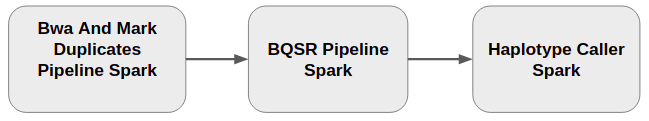
\includegraphics[scale=0.6]{figure/preprocessing.png}
\end{center}
\caption{Preprocessing steps in GATK 4.0~\label{preprocessing}}
\end{figure}

\subsection{Requirements Satisfaction}
The first step, BwaAndMarkDuplicatesPipelineSpark, differently by previous version tools, requires only one input file. Indeed while previously two paired end FASTQ files were accepted as input, now GATK prefers using an \textit{unmapped BAM} (uBAM) file format. So before of executing these commands, a further preprocessing is required: through the Picard tool FastqToSam is possible to convert two FASTQ files in a single uBAM file.\newline
Moreover, the reference genome indexes used in previous GATK versions are not enough: indeed it is required an other file in the folder containing the reference genome, a .fasta.img file. It is possible to create it through BwaMemIndexImageCreator.\newline
The following tools, BQSRPipelineSpark and HaplotypeCallerSpark, in addition to parameters described in Background chapter, require an other file in the reference folder, a .2bit file. For the reference genome HG19 used in this project, it is possible to download it from Internet.

\subsection{Pipeline Implementation}
After satisfying the requirements, there are two approaches to implement the Preprocessing phase: GATK 4.0 and Integrated Pipeline:
\begin{enumerate}
  \item \textbf{GATK 4.0}: a bash script that calls the Pipelines commands sequentially, executing the first command on every input sample (a for loop), for then continuing this approach with following tools.
So with the tools illustrated in Figure \ref{preprocessing} it is possible to execute this part of the pipeline for many input samples; after that, the outputs generated for each sample will be used as input for GenotypeGVCFs, for then executing the Variant Calling.\newline
With this approach, this part of the pipeline will produce 2 intermediate files that will cause disk access.

  \item \textbf{Integrated Pipeline}: ; in this approach was attempted to avoid intermediate disk access. Deepening the Java code of tools \href{https://github.com/broadinstitute/gatk/blob/9e4e41cbf2740ec3e5d41a5d3bbf9365bb2b51dd/src/main/java/org/broadinstitute/hellbender/tools/spark/pipelines/BwaAndMarkDuplicatesPipelineSpark.java}{BwaAndMarkDuplicatesPipelineSpark}, \href{https://github.com/broadinstitute/gatk/blob/81c9dc49eb630abf723c24d763f9ee1eb13028c1/src/main/java/org/broadinstitute/hellbender/tools/spark/pipelines/BQSRPipelineSpark.java}{BQSRPipelineSpark} and \href{https://github.com/broadinstitute/gatk/blob/8d929ed89984137fc00009b322074f7a0908d2a5/src/main/java/org/broadinstitute/hellbender/tools/HaplotypeCallerSpark.java}{HaplotypeCallerSpark}, and exploring their class code, is possible to notice that each of these class is made of different JavaRDD which pass their output to the following JavaRDD, with a disk writing of the final result. So instead of writing on the file system the result of \href{https://github.com/broadinstitute/gatk/blob/9e4e41cbf2740ec3e5d41a5d3bbf9365bb2b51dd/src/main/java/org/broadinstitute/hellbender/tools/spark/pipelines/BwaAndMarkDuplicatesPipelineSpark.java}{BwaAndMarkDuplicatesPipelineSpark} for instance, it may be used as input of the first JavaRDD of BQSRPipelineSpark and so on, pipelining JavaRDDs. In this way it would be possible to avoid some of the intermediate writings. I asked about a possible design like this in \href{https://gatkforums.broadinstitute.org/gatk/discussion/comment/43588#Comment_43588}{GATK Forum}. They agree that this solution would avoid part of the heavy process of disk access, but they are still benchmarking whether is convenient or not having the entire solution in memory.\newline
I tried to produce a solution that follows this approach; observing at the tool output, is possible to notice that the BWA runs normally. After some time started the BQSR normal output, alternating to the BWA output (the two tools start working in parallel), for then raising an exception:
\begin{lstlisting}[language=Java,caption={Sequence Dictionary}]
java.lang.IllegalArgumentException: 
Reference index for 'chr4' not found in sequence dictionary.
\end{lstlisting}
suggesting a conflict of a reference index inside the sequence dictionary. After sharing the problem of this approach in the \href{https://gatkforums.broadinstitute.org/gatk/discussion/comment/43704#Comment_43704}{GATK Forum}, an issue in their Git Hub project was open. But I think that to carry out this approach will take much more time. I have not enough knowledge in this domain in order to achieve it. So I continued to use the only tools provided by GATK, without apporting any alteration.
\end{enumerate}


\section{Variant Discovery}
The approach used here is already exposed in Background chapter. Since that GATK does not provide Spark tools, for this phase has been used GATK v3.8-0, because this version provide complete tools (it will be clearer in a few lines).
After that all samples reached the HaplotypeCallerSpark step, are ready for the Variant Discovery phase and so apply the GenotypeGVCFs: this tool takes in input all files generated by HaplotypeCallerSpark executions and creates an output to be used for following steps; in particular this tool requires of an index, but the GATK v3.8 creates the index himself (this reason leads to choice GATK v3.8).\newline
After that is necessary to calculate and then apply Variant Recalibration for SNP before and INDEL later. All theses tasks are sequential and require few time compared to Preprocessing phase.

\section{Call Set Refinement}
This phase was already discussed in the Background chapter, here will be expressed more details. This phase starts with the output generated by the Variant Discovery phase. As GATK Best Practices suggests, it is necessary to execute sequentially these tools: CalculateGenotypePosteriors, VariantFiltration and VariantAnnotator.\newline
After that GATK Best Practices provide only some guidelines, because GATK does not cover following steps. So the last generated file (from VariantAnnotator) will be used by SelectVariants to create as many files as the input samples in Preprocessing phase. Each of these new files will be then processed by ANNOVAR and IGM Anno; and finally an Exonic Filter will be applied.\newline
In particular to apply annotation of ANNOVAR and IGM Anno have been used the same proceedings of a previous project. Before of applying ANNOVAR annotation, this software requires some human Databases relative to the reference genome used in the pipeline. ANNOVAR provides tools in order to download them and after that is possible to annotate variants.

\section{\textit{Sparkifying} not-Spark tools}
At this point is possible to see the entire pipeline at Figure \ref{NGS_Pipeline_GATK} (GATK tools have been marked in \textit{italics}); it is possible to notice that only part of the Preprocessing phase uses Spark tools. But it was required that the entire pipeline is implemented in Spark, due to continuity of the system.
\\[1\baselineskip]
To achieve this task has been used the \textbf{Pipe} Transformation method provided by Spark. From the documentation, this method "pipe each partition of the RDD through a shell command, e.g. a Perl or bash script. RDD elements are written to the process's stdin and lines output to its stdout are returned as an RDD of strings". In other words, it allows to execute inside Spark a software which is inside a Bash script. Since that to call each GATK tool must be used a bash command, with this method is possible to \textit{"import"} all the other tools in Spark.
\\[1\baselineskip]
For tools like \textit{FastqToSam}, this approach may introduce parallelism; indeed as observable in Figure \ref{NGS_Pipeline_GATK}, this tool must process each input sample in order to convert it in a uBAM file. As there are multiple samples in input, Spark will parallelise the conversion.\newline
There is an inconvenient: as this method receive in input a bash script, this must be saved on the File System. It means that it works only when executed in local on a single node. When executed in cluster mode, a \textit{FileNotFoundException} will be raised. So the parallelism level of this approach is limited to the only number of cores of the local machine, does not scale to the number of nodes in the cluster. As further development, it may be found a way to scale this tool in a cluster.
\\[1\baselineskip]
Referring to Figure \ref{NGS_Pipeline_GATK}, the remaining tools after Preprocessing phase (for how has been defined in this project) are not implemented in Spark. So has been adopted the same approach used for \textit{FastqToSam}: calling each tool through bash command inside the Pipe command. As possible to notice in Figure \ref{NGS_Pipeline_GATK}, tools from \textit{GenotypeVCFs} to \textit{SelectVariants} are execute only "one time" in the entire pipeline and not for each input sample as previous tools. It means that using Pipe will not lead any effective speed-up to the process. But as already exposed, a continuity solution was required.
\\[1\baselineskip]
After splitting the VCF file in many files as input samples through \textit{SelectVariants}, following tools must process many files. Here the pipeline gains a speed-up similar to the one gained with \textit{FastqToSam}. Since that ANNOVAR and IGM Anno tools are programmed in Perl language, it is possible to use the Perl command inside Pipe function and import this tools in Spark.\newline
The Exonic Filter is a simple filter which filters the input TSV file rows, according to specific rules. To create this function, Spark offers the method Filter, which is enough to achieve this task.
\\[1\baselineskip]
All these \textit{Sparkified} tools are written in Java using three classes:
\begin{enumerate}
  \item \textbf{FastqToSam}: encapsulates the \textit{FastqToSam} tool, requiring in input the Picard jar path, comma separated input files (the paired end fastq files to be converted in uBAM) and an output folder path. 
  \item \textbf{VariantDiscovery}: here have been encapsulated the Variant Discovery tools, so referring to Figure \ref{NGS_Pipeline_GATK}, are included tools from \textit{GenotypeVCFs} to \textit{INDEL Recalibration}, which means that this part is without speed-up.
  \item \textbf{CallsetRefinement}: this class encapsulates tools from \textit{Genotype Refinement} to the \textit{Exonic Filter}. As exposed before, the part after \textit{SelectVariants} gains speed-up.
\end{enumerate}
All three classes extend an Abstract Class which provides them support methods such as creating an executable bash script on the file system, executing bash commands, locating required input files on the file system.\newline
The choice to include all the Variant Discovery and Call Set Refinement tools in two classes is due to give more flexibility to the user of these tools; indeed to execute respectively Variant Discovery and Call Set Refinement tools will be necessary to use only two bash command. These classes are callable through the \textit{spark-submit} script provided inside the Spark package.
\\[2\baselineskip]
At this point the entire pipeline meant to run on a local machine can be expressed as a bash script. This will contain a spark-submit calling FastqToSam class, \textit{for loops} respectively for BwaAndMarkDuplicatesPipelineSpark, BQSRPipelineSpark and HaplotypeCallerSpark, processing each sample; two spark-submit calling respectively VariantDiscovery and CallsetRefinement.\newline
The generated output files have been compared with a previous similar pipeline \cite{ScalableEfficientWhole-ExomeProcessing} results and they are much similar; it should be necessary only to apply an higher filter in VariantFiltration.

\begin{sidewaysfigure}
\begin{center}
    \centering
	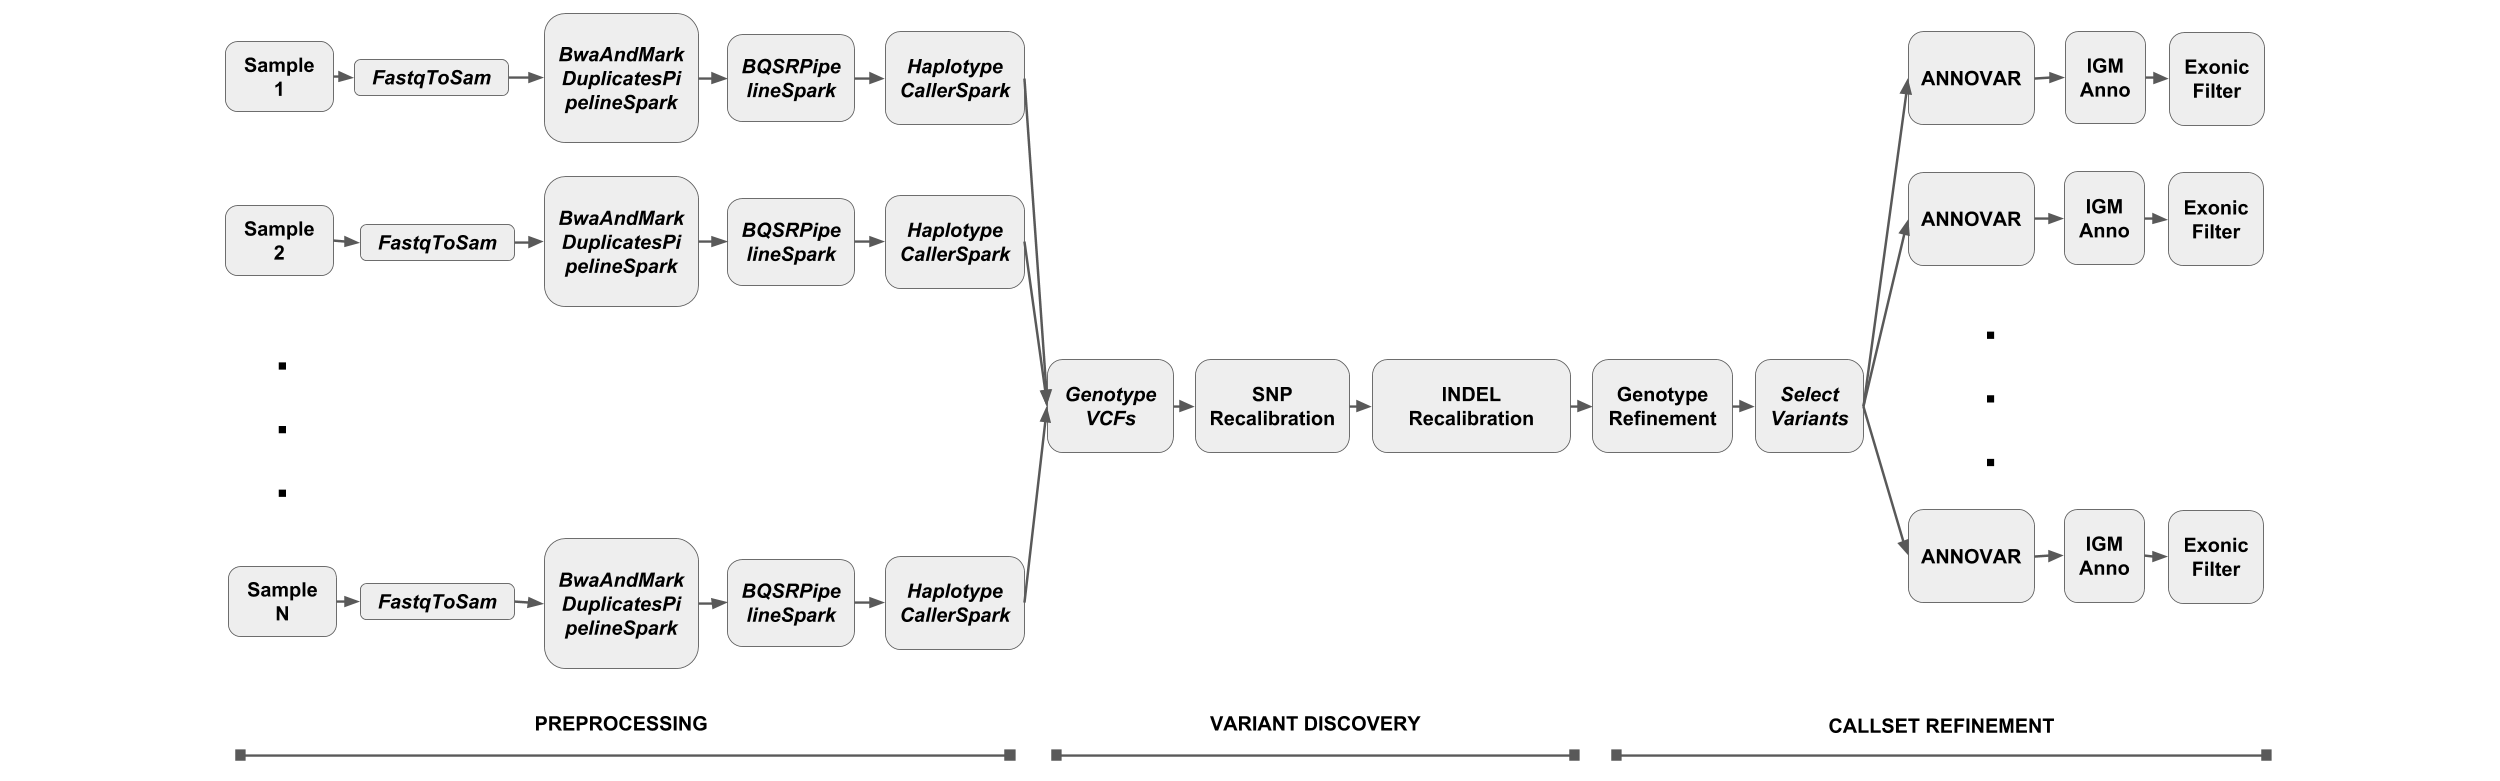
\includegraphics[scale=0.245]{figure/NGS_Pipeline_GATK.png}
    \caption{NGS Pipeline~\label{NGS_Pipeline_GATK}}
\end{center}
\end{sidewaysfigure}









